
\section{Advanced gradient-based edgedetection}
\begin{frame}
	\frametitle{Prewitt Operator}
	\begin{center}
		Idea: Include neighboorhood
	\end{center}
	~\newline
	\begin{columns}
		\begin{column}{0.5\textwidth}
			\begin{center}
				$H^P_x = \begin{bmatrix}
				-1 & 0 & 1 \\ -1 & 0 & 1 \\ -1 & 0 & 1
				\end{bmatrix} $
			\end{center}	
		\end{column}
		\begin{column}{0.5\textwidth} 
			\begin{center}
				$H^P_y = \begin{bmatrix}
				-1 & -1 & -1 \\ 0 & 0 & 0 \\ 1 & 1 & 1
				\end{bmatrix} $
			\end{center}
		\end{column}
	\end{columns}
	~\newline
	\begin{center}
		$\nabla I^P(u,v)\approx \dfrac{1}{6} \cdot \begin{pmatrix}
		(I\ast H^P_x)(u,v) \\ (I\ast H^P_y)(u,v) 
		\end{pmatrix}$
	\end{center}
\end{frame}
\begin{frame}
	\frametitle{Sobel}
	\begin{center}
		Idea: Include neighboorhood but weight center more
	\end{center}
	~\newline	
	\begin{columns}
		\begin{column}{0.5\textwidth}
			\begin{center}
				$H^S_x = \begin{bmatrix}
				-1 & 0 & 1 \\ -2 & 0 & 2 \\ -1 & 0 & 1
				\end{bmatrix} $
			\end{center}	
		\end{column}
		\begin{column}{0.5\textwidth} 
			\begin{center}
				$H^S_y = \begin{bmatrix}
				-1 & -2 & -1 \\ 0 & 0 & 0 \\ 1 & 2 & 1
				\end{bmatrix} $
			\end{center}
		\end{column}
	\end{columns}
	~\newline
	\begin{center}
		$\nabla I^S(u,v)\approx \dfrac{1}{8} \cdot \begin{pmatrix}
		(I\ast H^S_x)(u,v) \\ (I\ast H^S_y)(u,v) 
		\end{pmatrix}$
	\end{center}
\end{frame}
\begin{frame}
	\frametitle{Comparison with Felix}
	\begin{columns}
		\begin{column}{0.33\textwidth}
			\begin{figure}
				\centering
				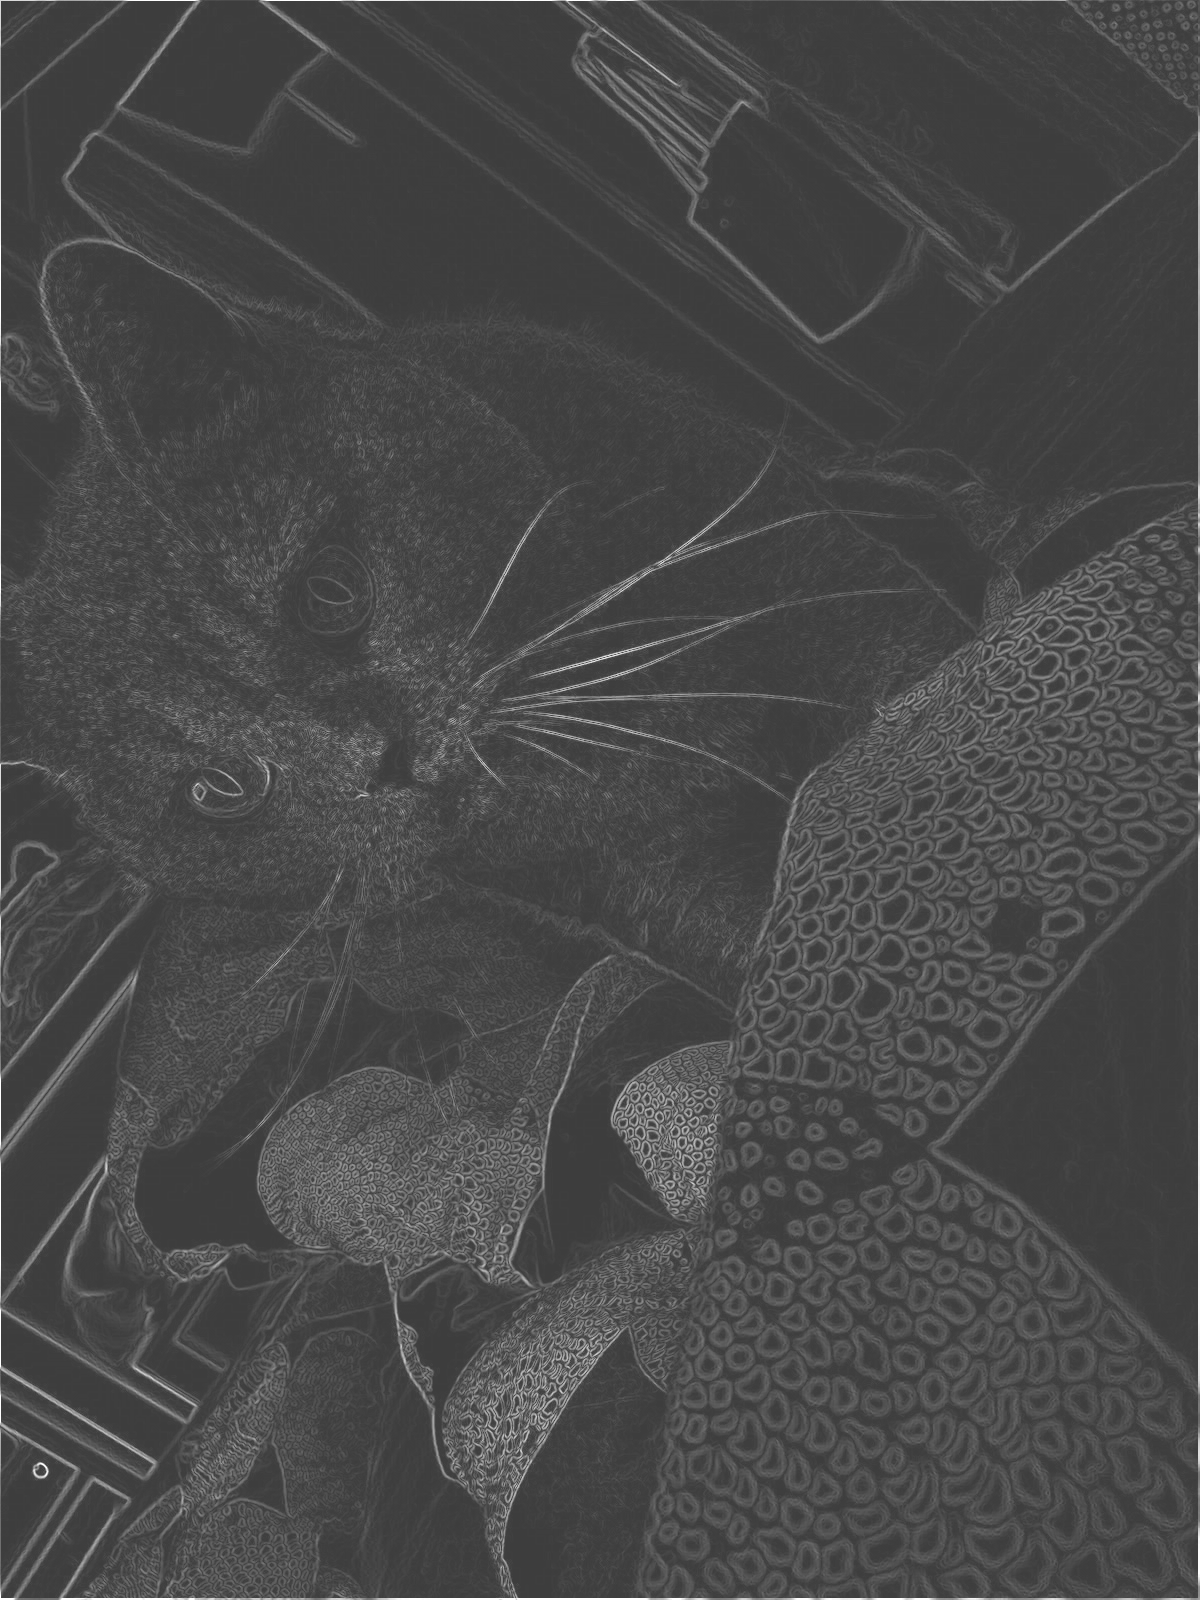
\includegraphics[width=0.8\linewidth]{images/KadseSimple}
				\caption[Simple edge filter]{Simple edge filter}
				\label{fig:Simple}
			\end{figure}
		\end{column}
		\begin{column}{0.33\textwidth}
				\begin{figure}
					\centering
					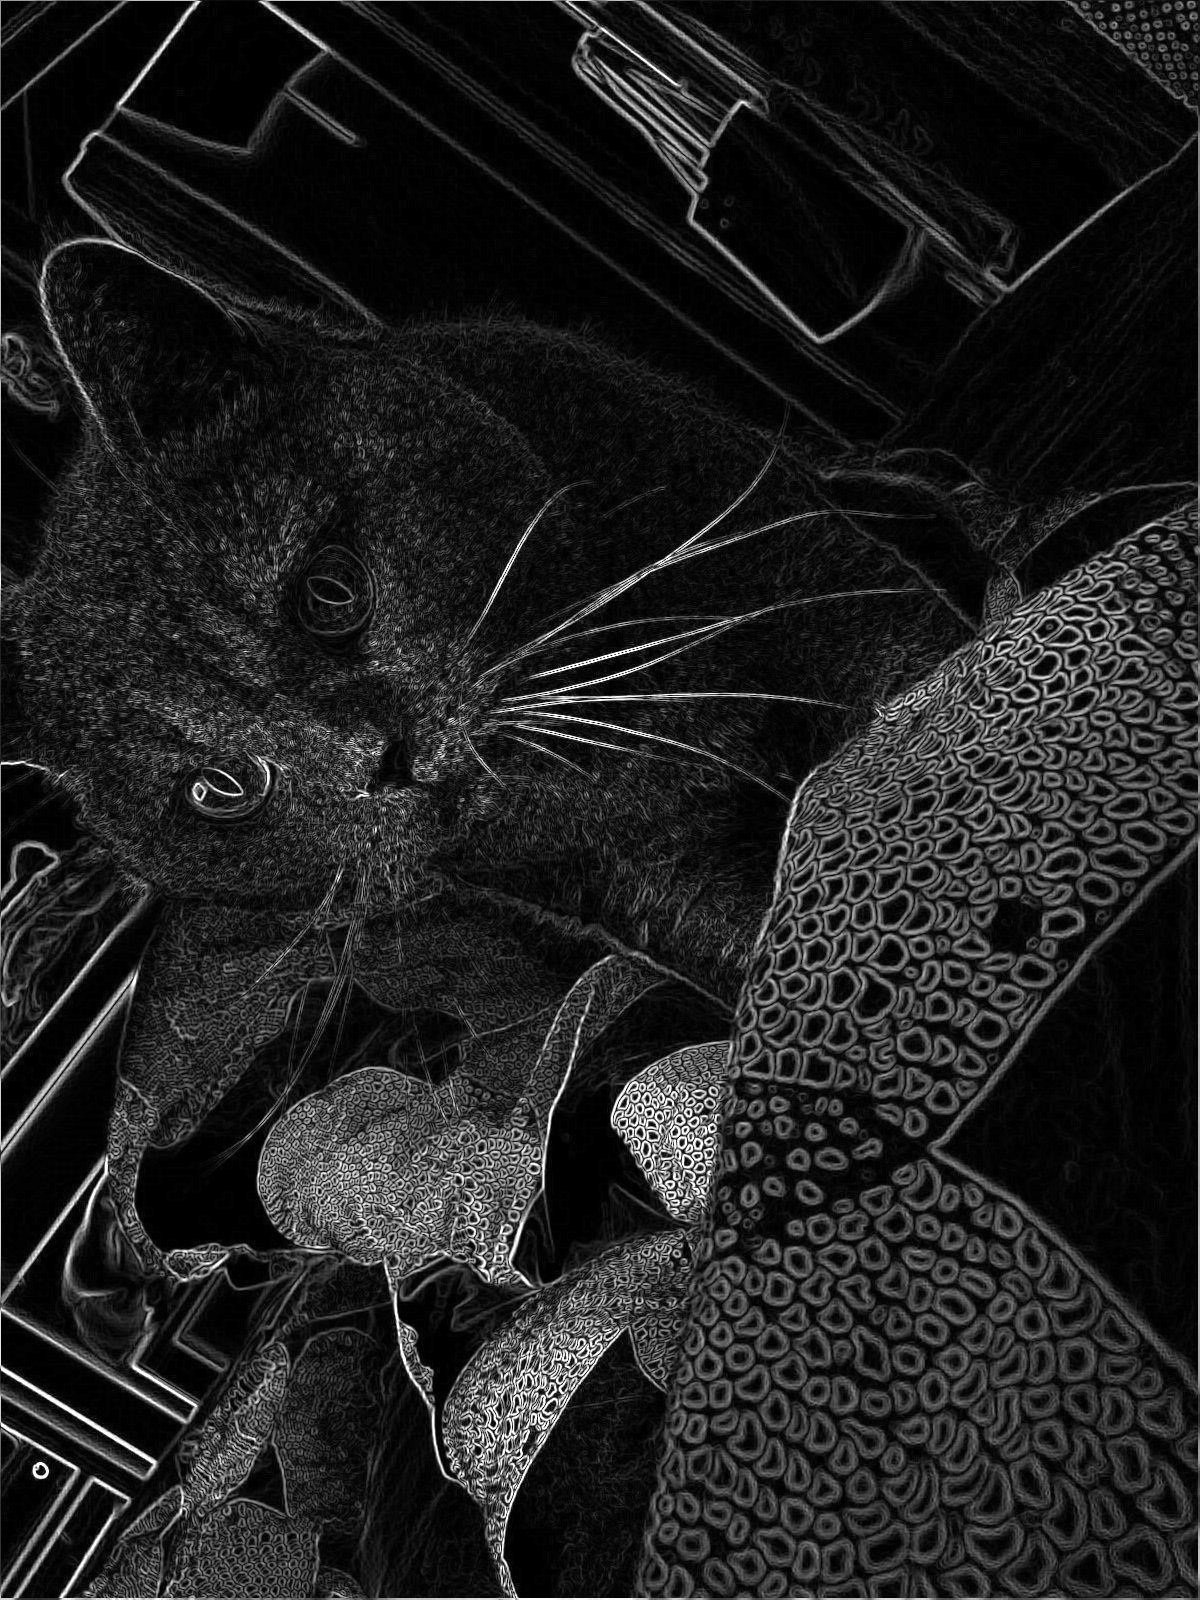
\includegraphics[width=0.8\linewidth]{images/KadsePrewitt}
					\caption[Prewitt Operator]{Prewitt Operator}
					\label{fig:KadsePrewitt}
				\end{figure}
		\end{column}
		\begin{column}{0.33\textwidth}
			\begin{figure}
				\centering
				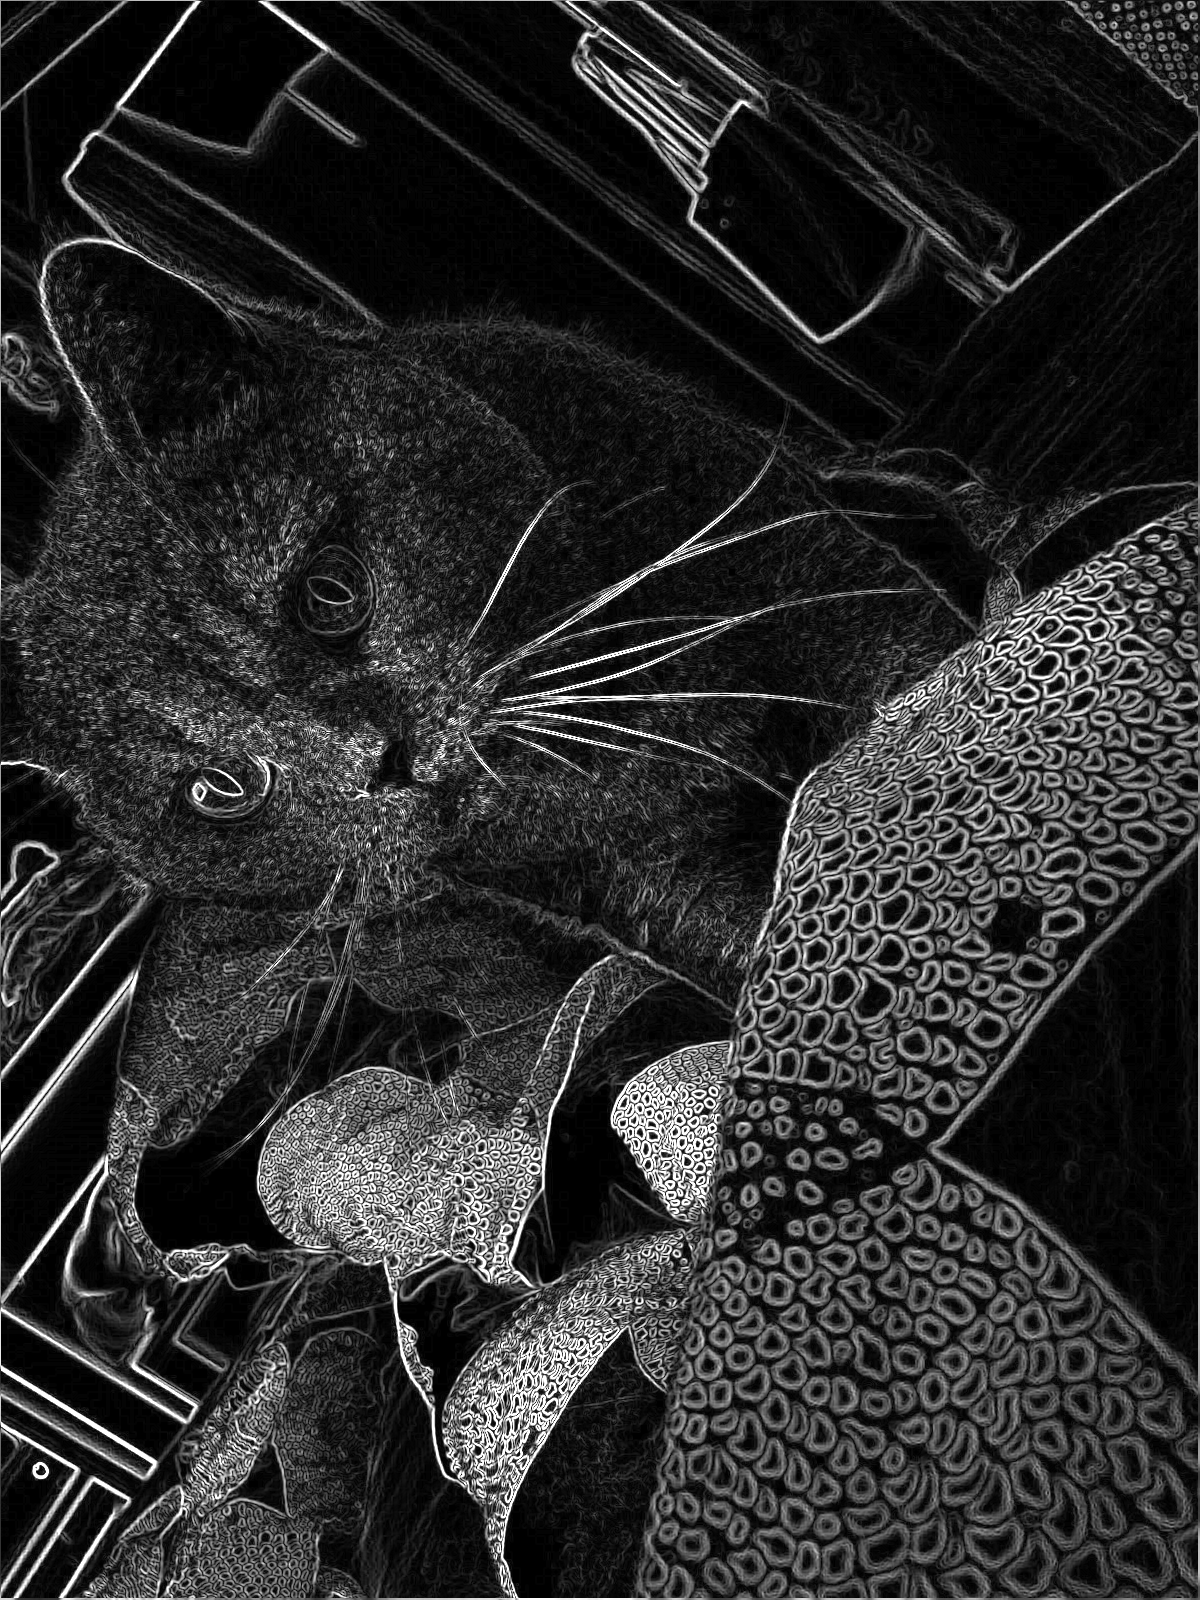
\includegraphics[width=0.8\linewidth]{images/KadseSobel}
				\caption[Sobel Operator]{Sobel Operator}
				\label{fig:KadseSobel}
			\end{figure}
		\end{column}
	\end{columns}
\end{frame}
\begin{frame}
	\frametitle{Evaluations}
	\begin{center}
		\textbf{general magnitude}: $E(u,v) = \sqrt{I_x^2(u,v)+I_y^2(u,v)}$
		\newline holds for every Operator 
		~\newline
		\begin{figure}
			\centering
			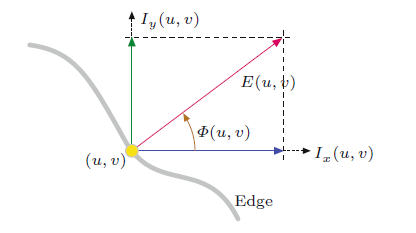
\includegraphics[width=0.5\linewidth]{images/EdgeDirection}
			\caption[Visualisation of edge direction]{Visualisation of edge direction}
			\label{fig:edgedir}
		\end{figure}
		~\newline
		$\Phi(u,v)=\tan^{-1}\left(\dfrac{I_y(u,v)}{I_x(u,v)}\right)=\arctan(I_x(u,v),I_y(u,v))$
	\end{center}
	
\end{frame}

\section{Compass Operators}
\begin{frame}
\frametitle{Compass Operators}
\begin{columns}
	\begin{column}{0.69\textwidth}
		\textbf{Problem:} The stronger a filter responses to edge-like structures, the more sensitive it is to orientation \newline
		$\Uparrow Orientation \approx \Downarrow Edges$ $ \Uparrow Edges \approx \Downarrow Orientation $ \newline
		\textbf{Solution:} Apply 8 filters for each direction of the compass ~\newline \textbf{Produce two pictures:} One for the edge-strength taking the magnitude of the strongest activated filter, ~\newline one for the direction marking the strongest filter with colour 
	\end{column}
	\begin{column}{0.29\textwidth}
		\begin{figure}
			\centering
			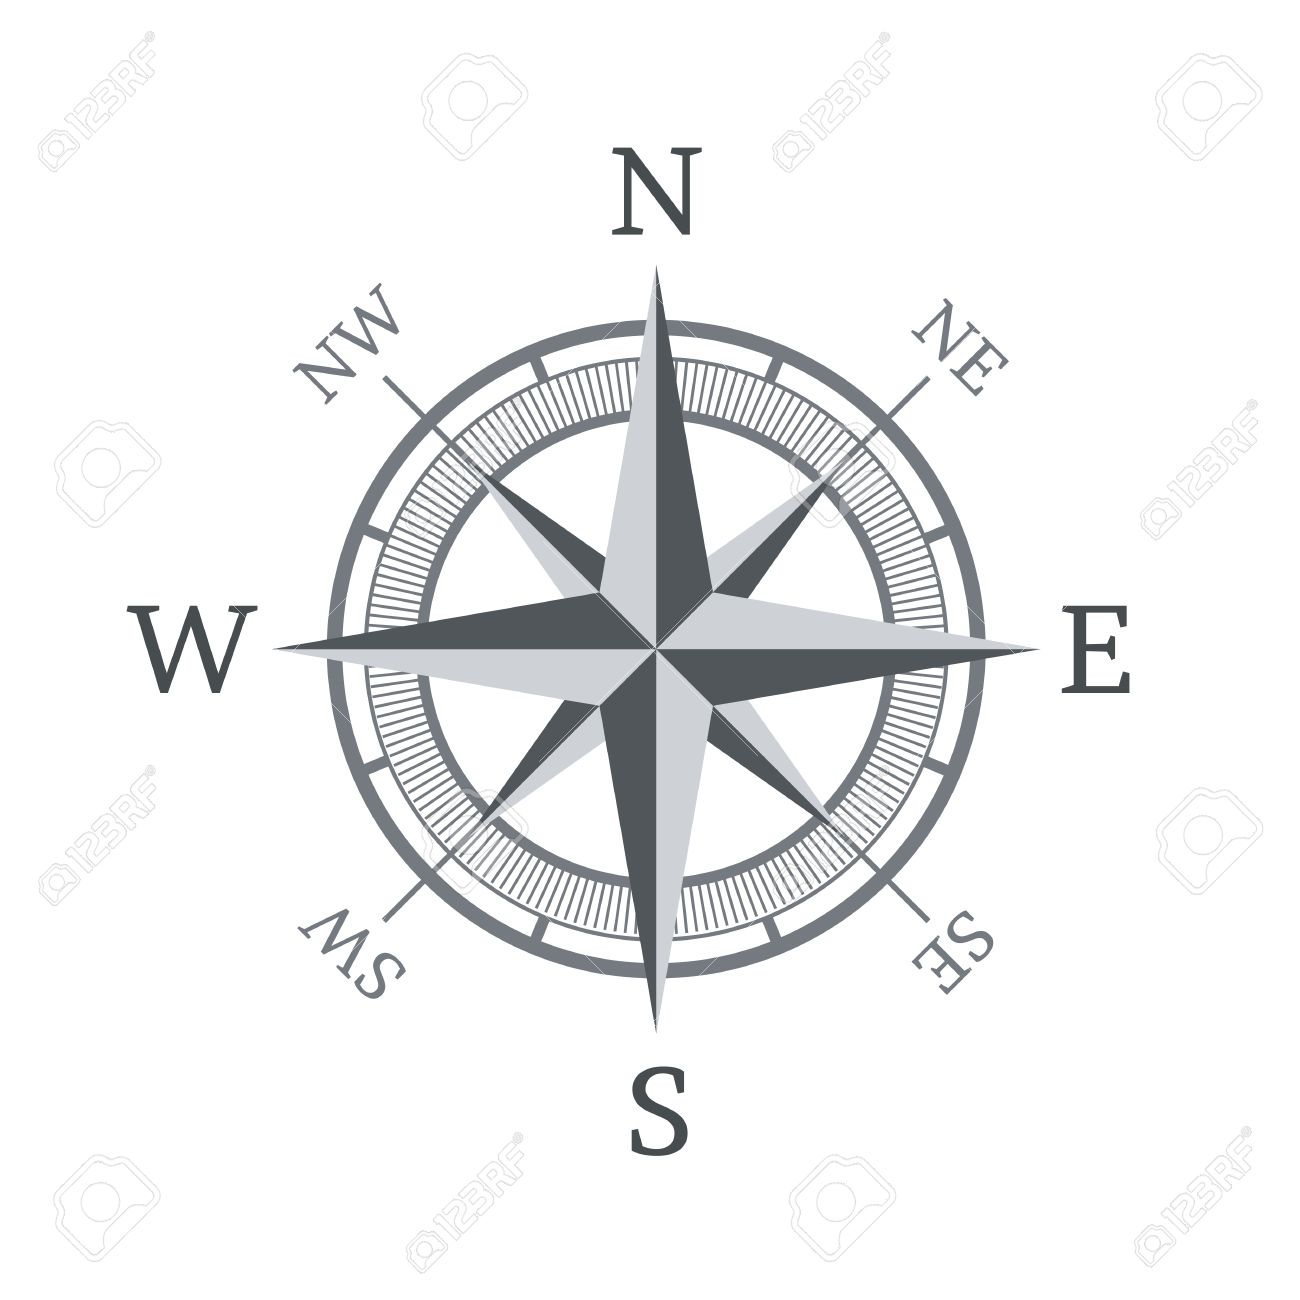
\includegraphics[width=0.45\textwidth]{images/Kompass}
			\label{fig:Kompass}
		\end{figure}
	\end{column}	
\end{columns}
\end{frame}

\begin{frame}
\frametitle{Extended Sobel Operator}
\begin{columns}
\begin{column}{0.6\textwidth}
	\begin{figure}
		\centering
		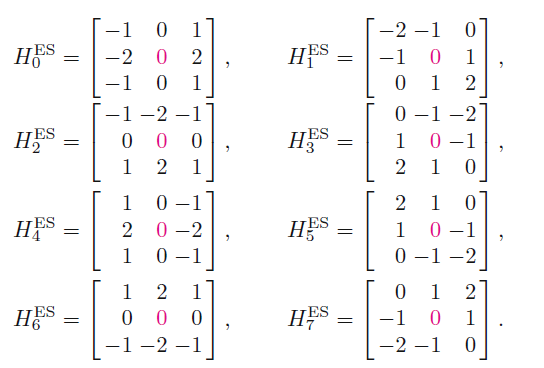
\includegraphics[width=0.8\linewidth]{images/ExtendedSobel}
		\caption[Extended Sobel Operator]{Extended Sobel Operator}
		\label{fig:ESobel}
	\end{figure}
\end{column}
\begin{column}{0.4\textwidth}
	Note: Its only required to apply 4 filters, as they are symetric
\end{column}
\end{columns}
\end{frame}

\begin{frame}
\frametitle{Extended Sobel Example}
\begin{columns}
\begin{column}{0.5\textwidth}
\begin{figure}
	\centering
	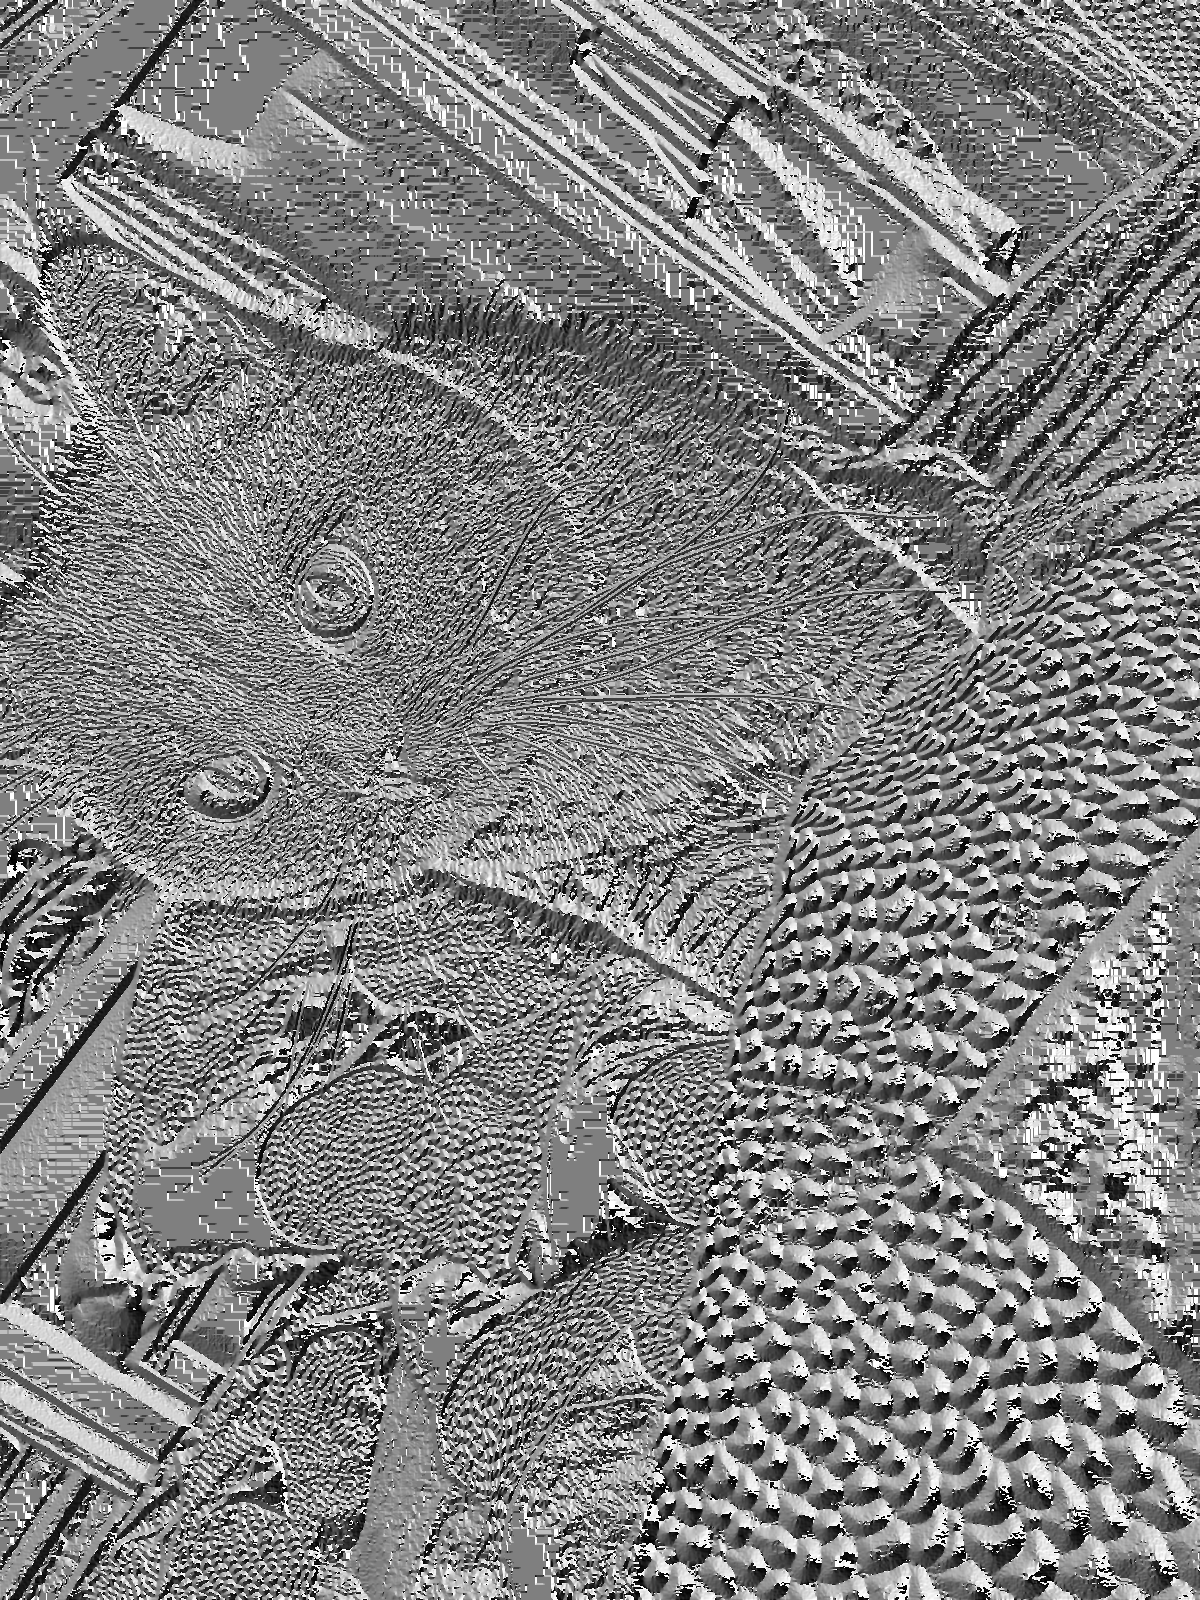
\includegraphics[width=0.8\linewidth]{images/PhiFelix}
	\caption[$\Phi^{ES}(Felix)$]{$\Phi^{ES}(Felix)$}
	\label{fig:PhiFelix}
\end{figure}
\end{column}
\begin{column}{0.5\textwidth}
\begin{figure}
	\centering
	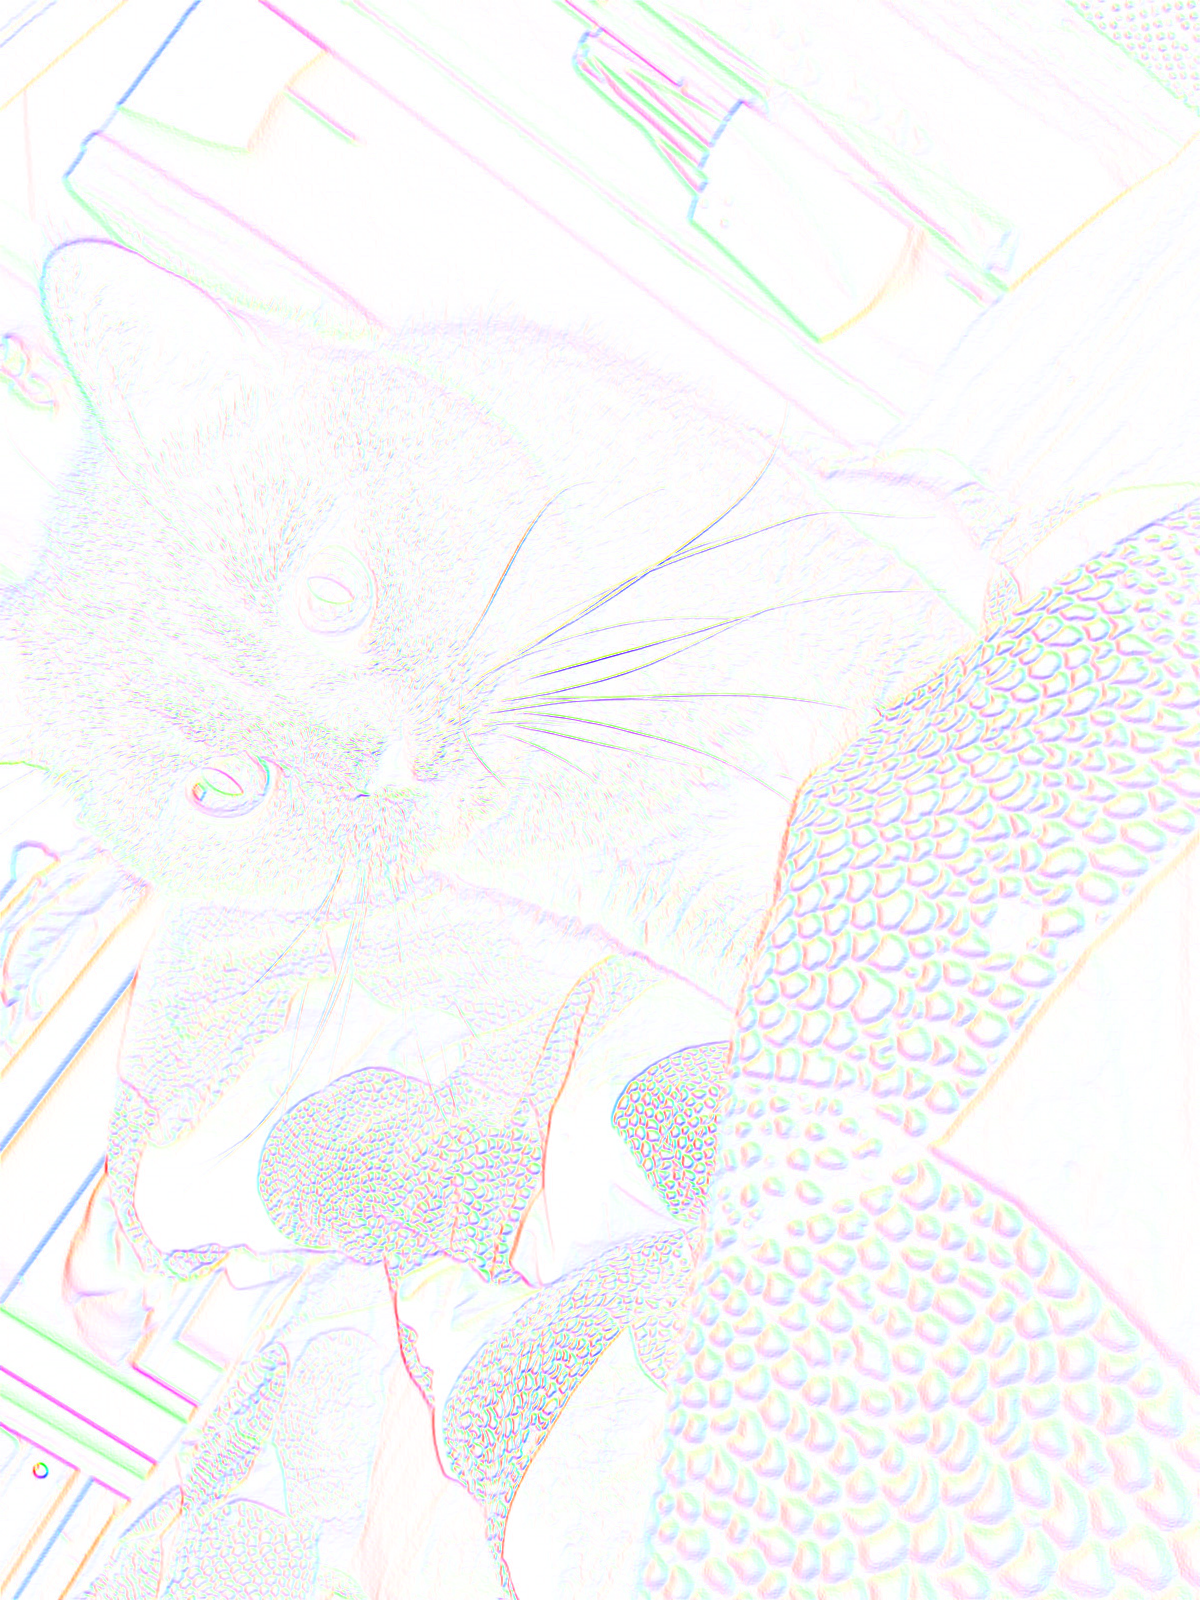
\includegraphics[width=0.8\linewidth]{images/PhiFelixColoured}
	\caption[Colour encoding]{Colour encoding}
	\label{fig:PhiFelixColour}
\end{figure}
\end{column}
\end{columns}
\end{frame}
\begin{frame}
\frametitle{Kirsch Operator}
\begin{columns}
\begin{column}{0.6\textwidth}
\begin{figure}
\centering
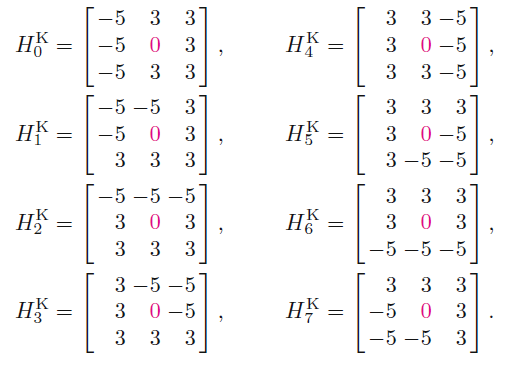
\includegraphics[width=0.8\linewidth]{images/KirschOperator}
\caption[Kirsch Operator]{Kirsch Operator}
\label{fig:Kirsch}
\end{figure}
\end{column}
\begin{column}{0.4\textwidth}
\begin{figure}
\centering
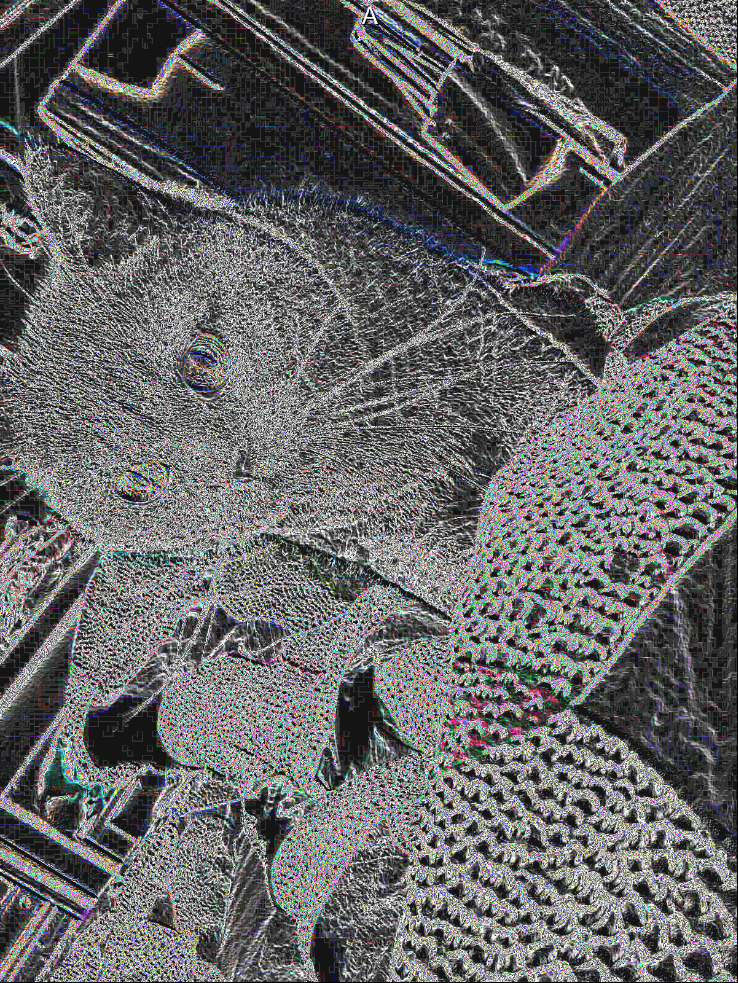
\includegraphics[width=0.8\linewidth]{images/KadseKirsch}
\caption[Felix with Kirsch]{Felix with Kirsch}
\label{fig:FelixKirsch}
\end{figure}
\end{column}
\end{columns}
\end{frame}